\chapter{Use cases}
%begin actors section
\section{Actors}
	The platform recognizes two type of actors in the first place, the unidentified user and the registered user.
	\subsection{Unidentified user}
		This actor has only registration and authentication rights on the platform.
	\subsection{Registered user}
		A register user has only one identity listed below.
		\subsubsection{Student}
			This actor has the rights to take exercises and be graded by the platform.
		\subsubsection{Teacher}
			This actor has the rights to supervise students such as providing exercises.
		\subsubsection{Administrator}
			This actor has the rights above and make sure things are running smoothly.
%end actors section
\newpage
%begin free user section
\section{Unidentified user}
	\subsection{Overview}
		\begin{figure}[ht]
			\begin{center}
				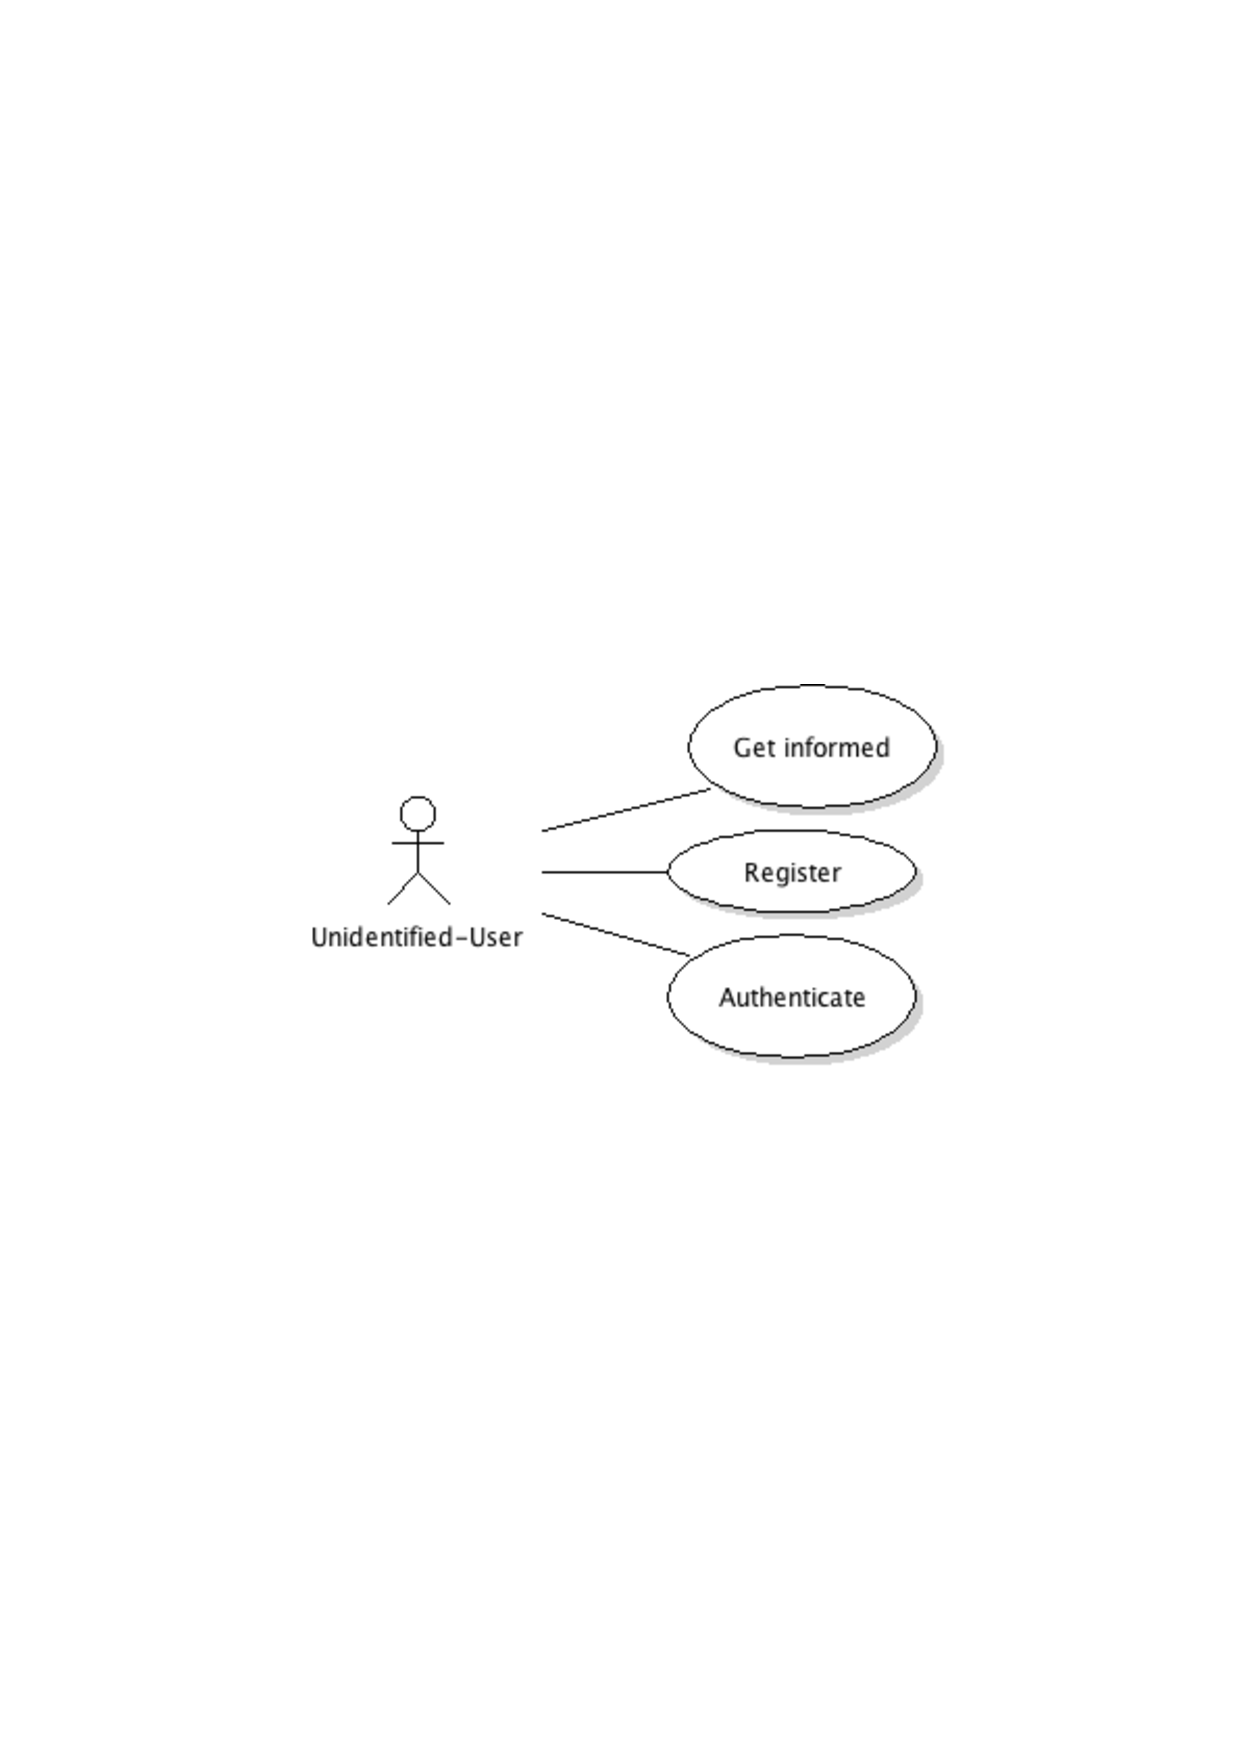
\includegraphics[width=\textwidth,  trim=2cm 12cm 2cm 11cm]{UML_figure/UC/uni_user/UC_UniUser_General.pdf}
				\caption{Unidentified user use cases : Overview}
			\end{center}
		\end{figure}
		\subsubsection{Get informed}An unidentified user gets informed about what the platform is.
		\subsubsection{Register}An unidentified user who wants to access to the platform has to register first.
		\subsubsection{Authenticate}An unidentified user authenticates to have access to the platform if the user is already registered.
%end free user section
\newpage
%begin student section
\section{Student}
	\subsection{Overview}
		\begin{figure}[ht]
			\begin{center}
				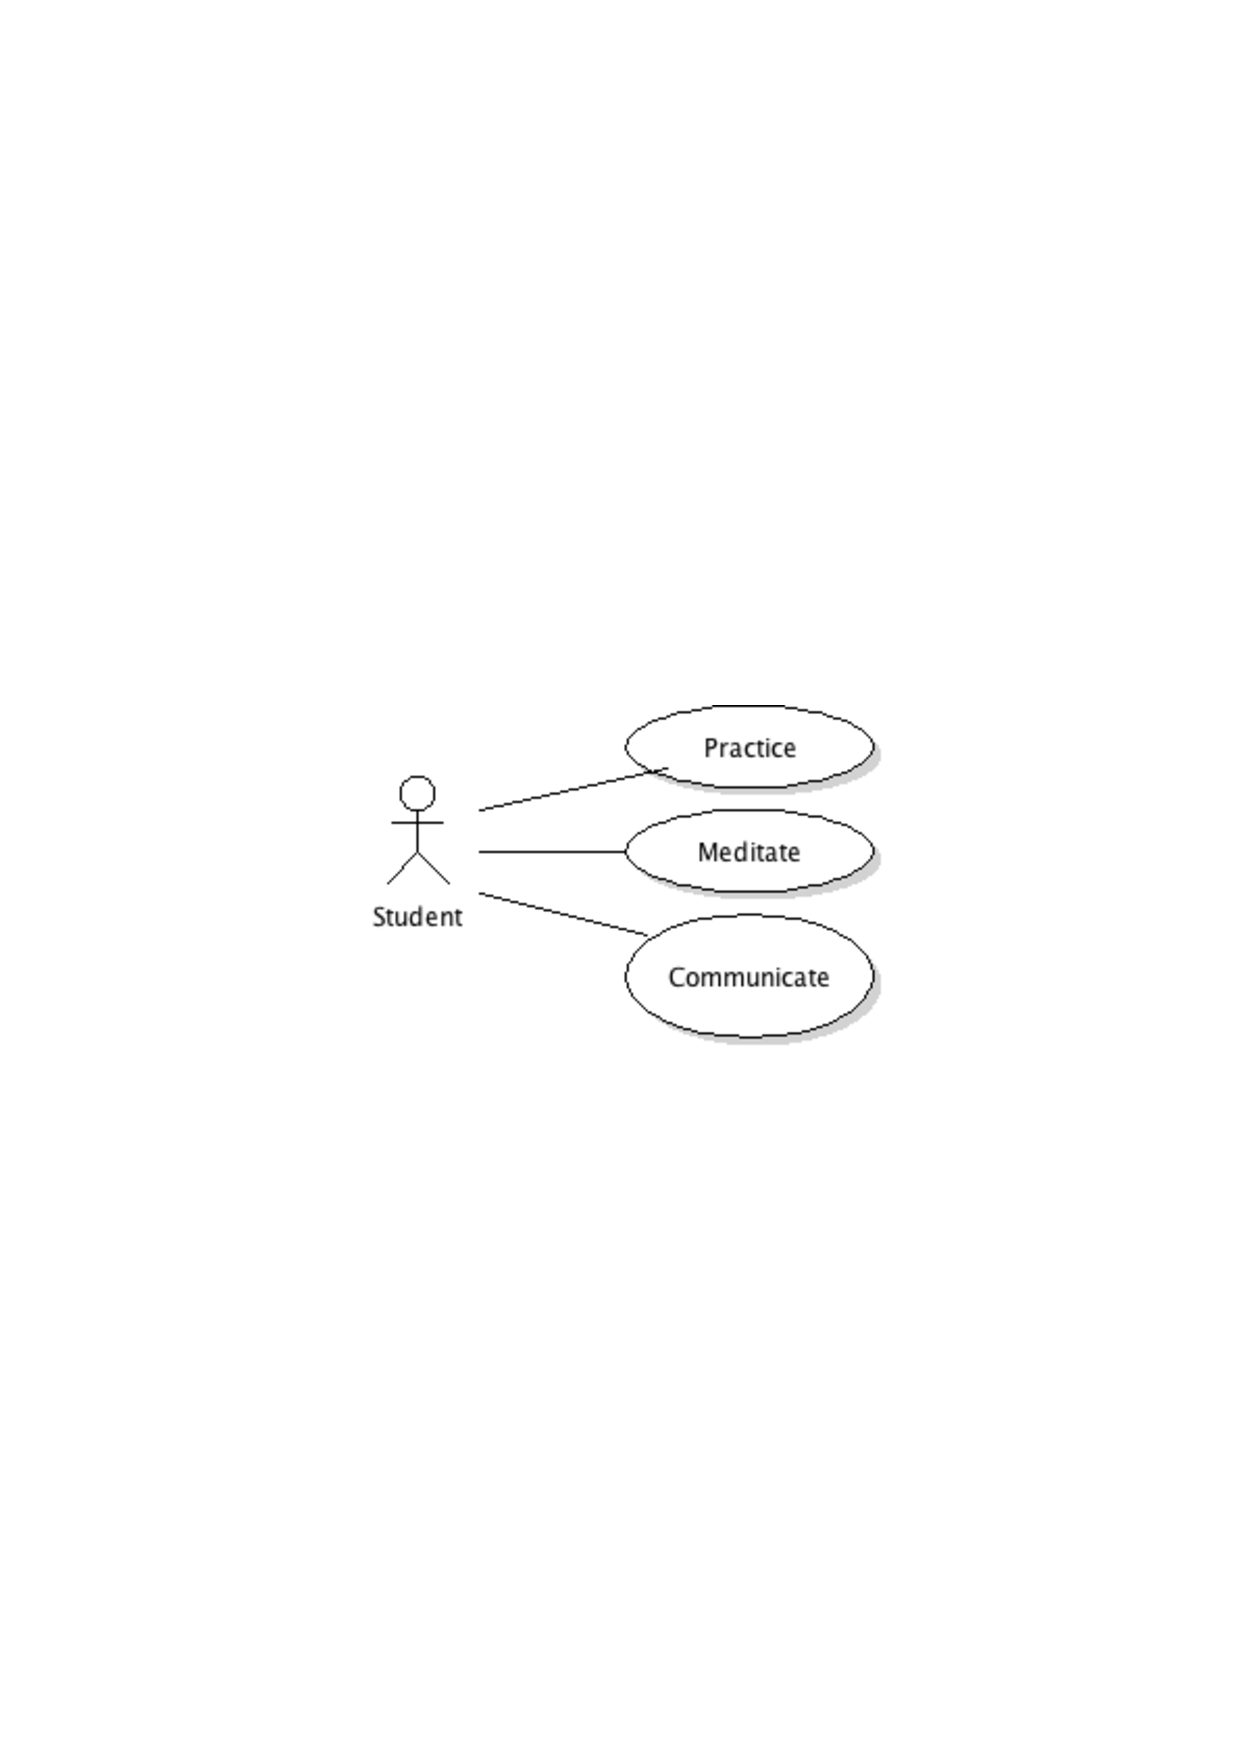
\includegraphics[width=\textwidth,  trim=2cm 12cm 2cm 12cm]{UML_figure/UC/student/UC_Student_General.pdf}
				\caption{Student use cases : Overview}
			\end{center}
		\end{figure}
		\subsubsection{Learn}
			The student learns her lessons and do exercises.
		\subsubsection{Meditate}
			The students meditates on her performances and overcomes her weaknesses by doing suggested exercises.
		\subsubsection{Communicate}
			The students communicates with authenticate users in order to fix her issue and to improve herself.
\newpage
	\subsection{Learn}
		\begin{figure}[ht]
			\begin{center}
				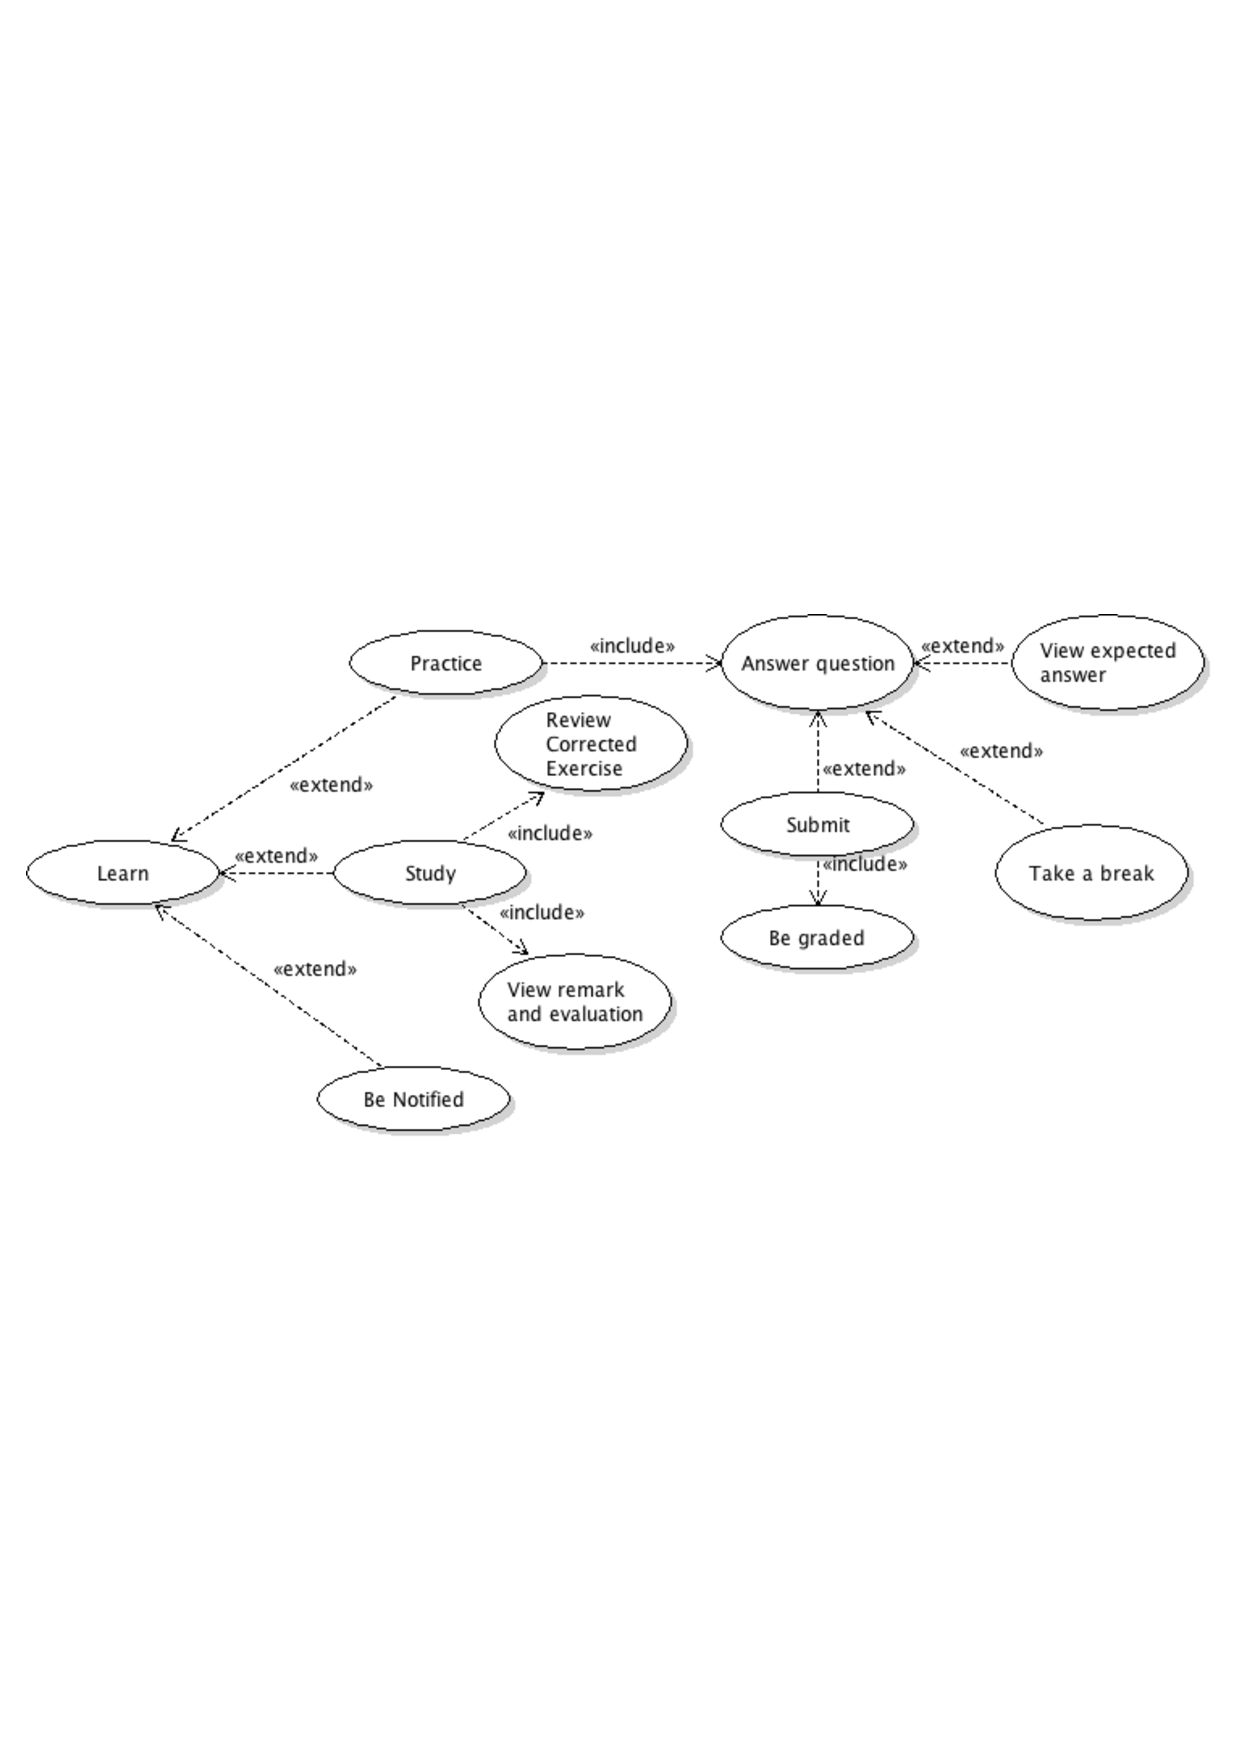
\includegraphics[width=\textwidth,  trim=2cm 10cm 2cm 8cm]{UML_figure/UC/student/UC_Student_Learn.pdf}
				\caption{Student use cases : Learn}
			\end{center}
		\end{figure}
		\subsubsection{Be notified}
			The student is notified for new events concerning her learning process.
		\subsubsection{Study}
			The student studies by reviewing corrected exercises.\\
			The student studies by reviewing teacher's evaluation and remarks.
		\subsubsection{Practice}
			The student practice her skills by answering questions.
		\subsubsection{Answer question}
			The student answers a set of questions.
		\subsubsection{View expected answer}
			The student has optionally access to the corrected version.
		\subsubsection{Take a break}
			The student takes a break and will resume the exercise later.
		\subsubsection{Submit}
			The student submit her answer form.
		\subsubsection{Be graded}
			The student is also graded by the platform \textit{after} she submits her answer form.		
	\subsection{Meditate}
		\begin{figure}[ht]
			\begin{center}
				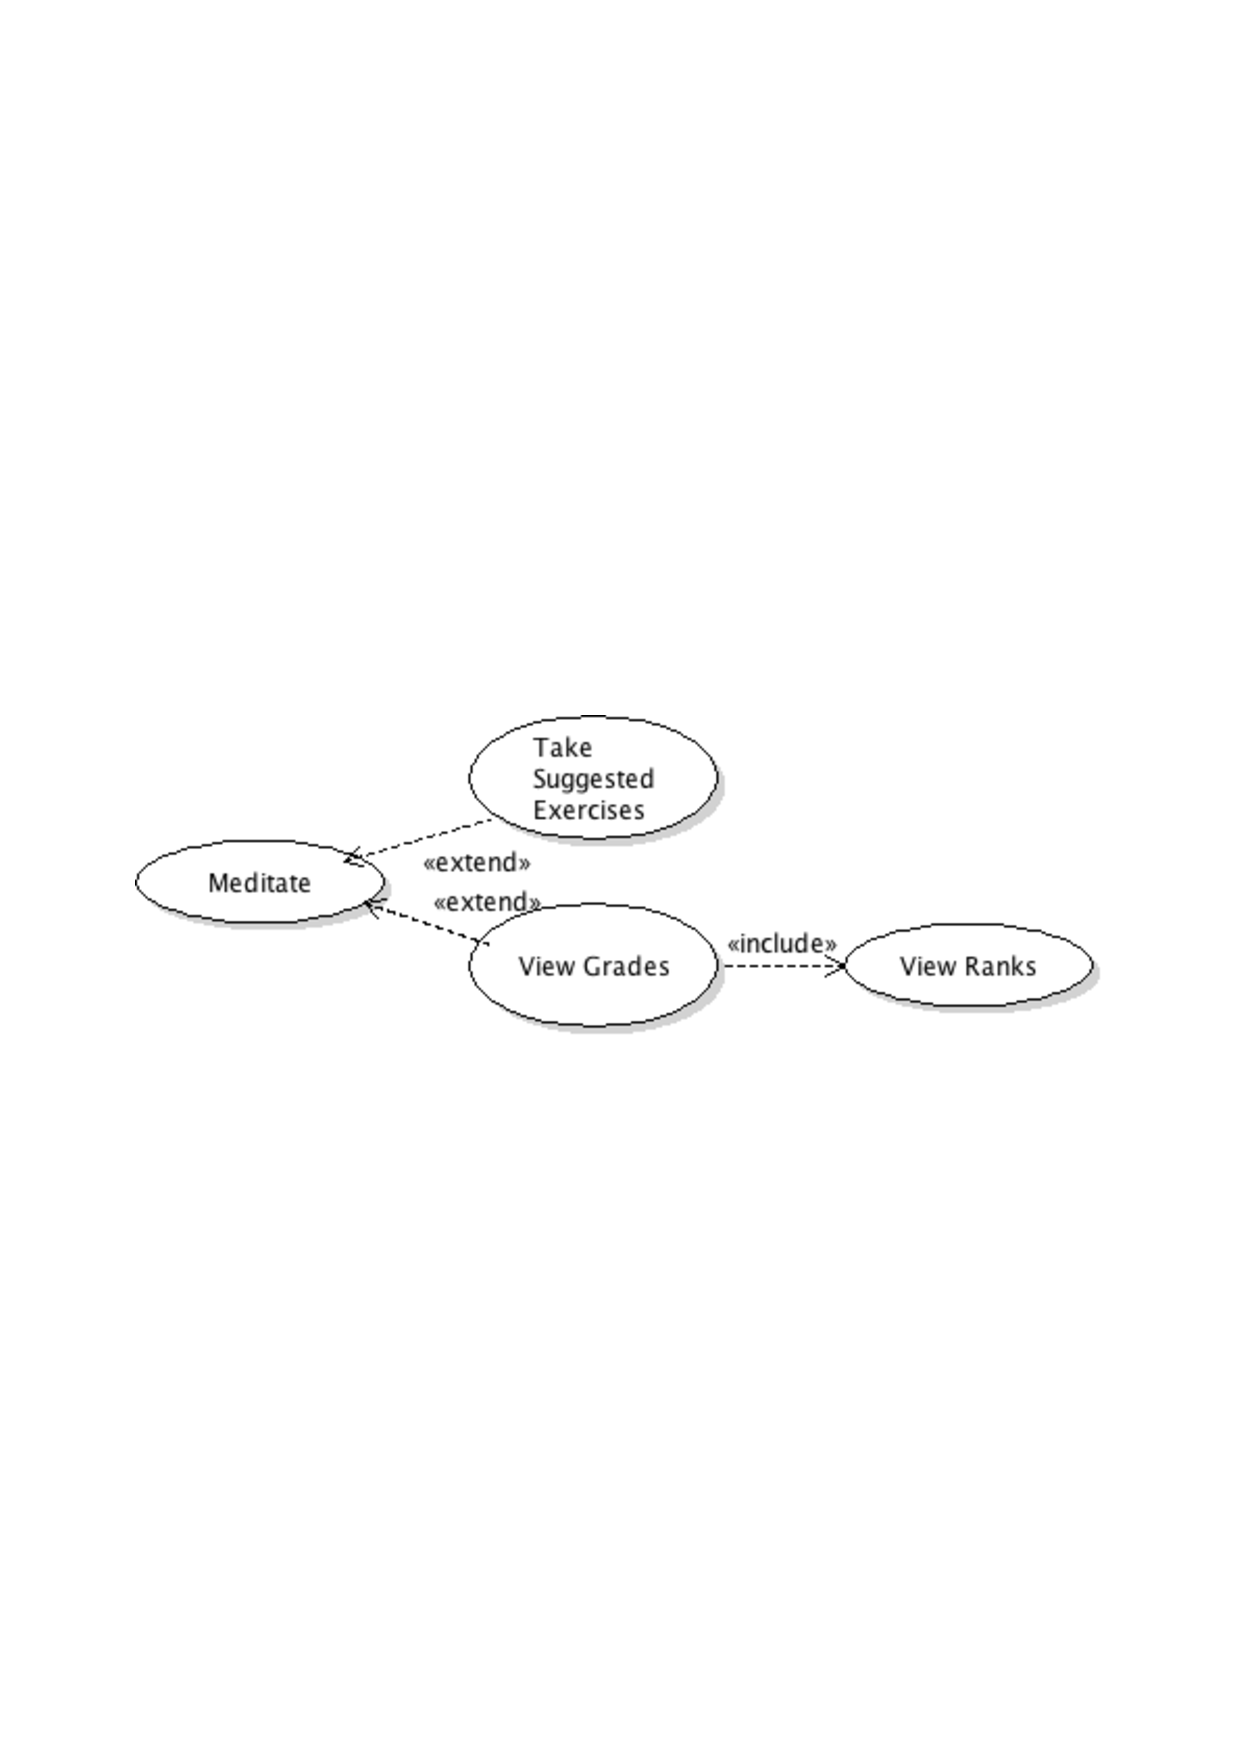
\includegraphics[width=\textwidth,  trim=2cm 12cm 2cm 12cm]{UML_figure/UC/student/UC_Student_Meditate.pdf}
				\caption{Student use cases : Meditate}
			\end{center}
		\end{figure}
		\subsubsection{Take suggested exercises}
			The student will be proposed exercises according to her grade.
		\subsubsection{View Grades}
			The student observe her grade for each exercises.
		\subsubsection{View Ranks}
			The student compares herself with other students.
%end student section
\newpage
%begin teacher section
\section{Teacher}
	\subsection{Overview}
		\begin{figure}[ht]
			\begin{center}
				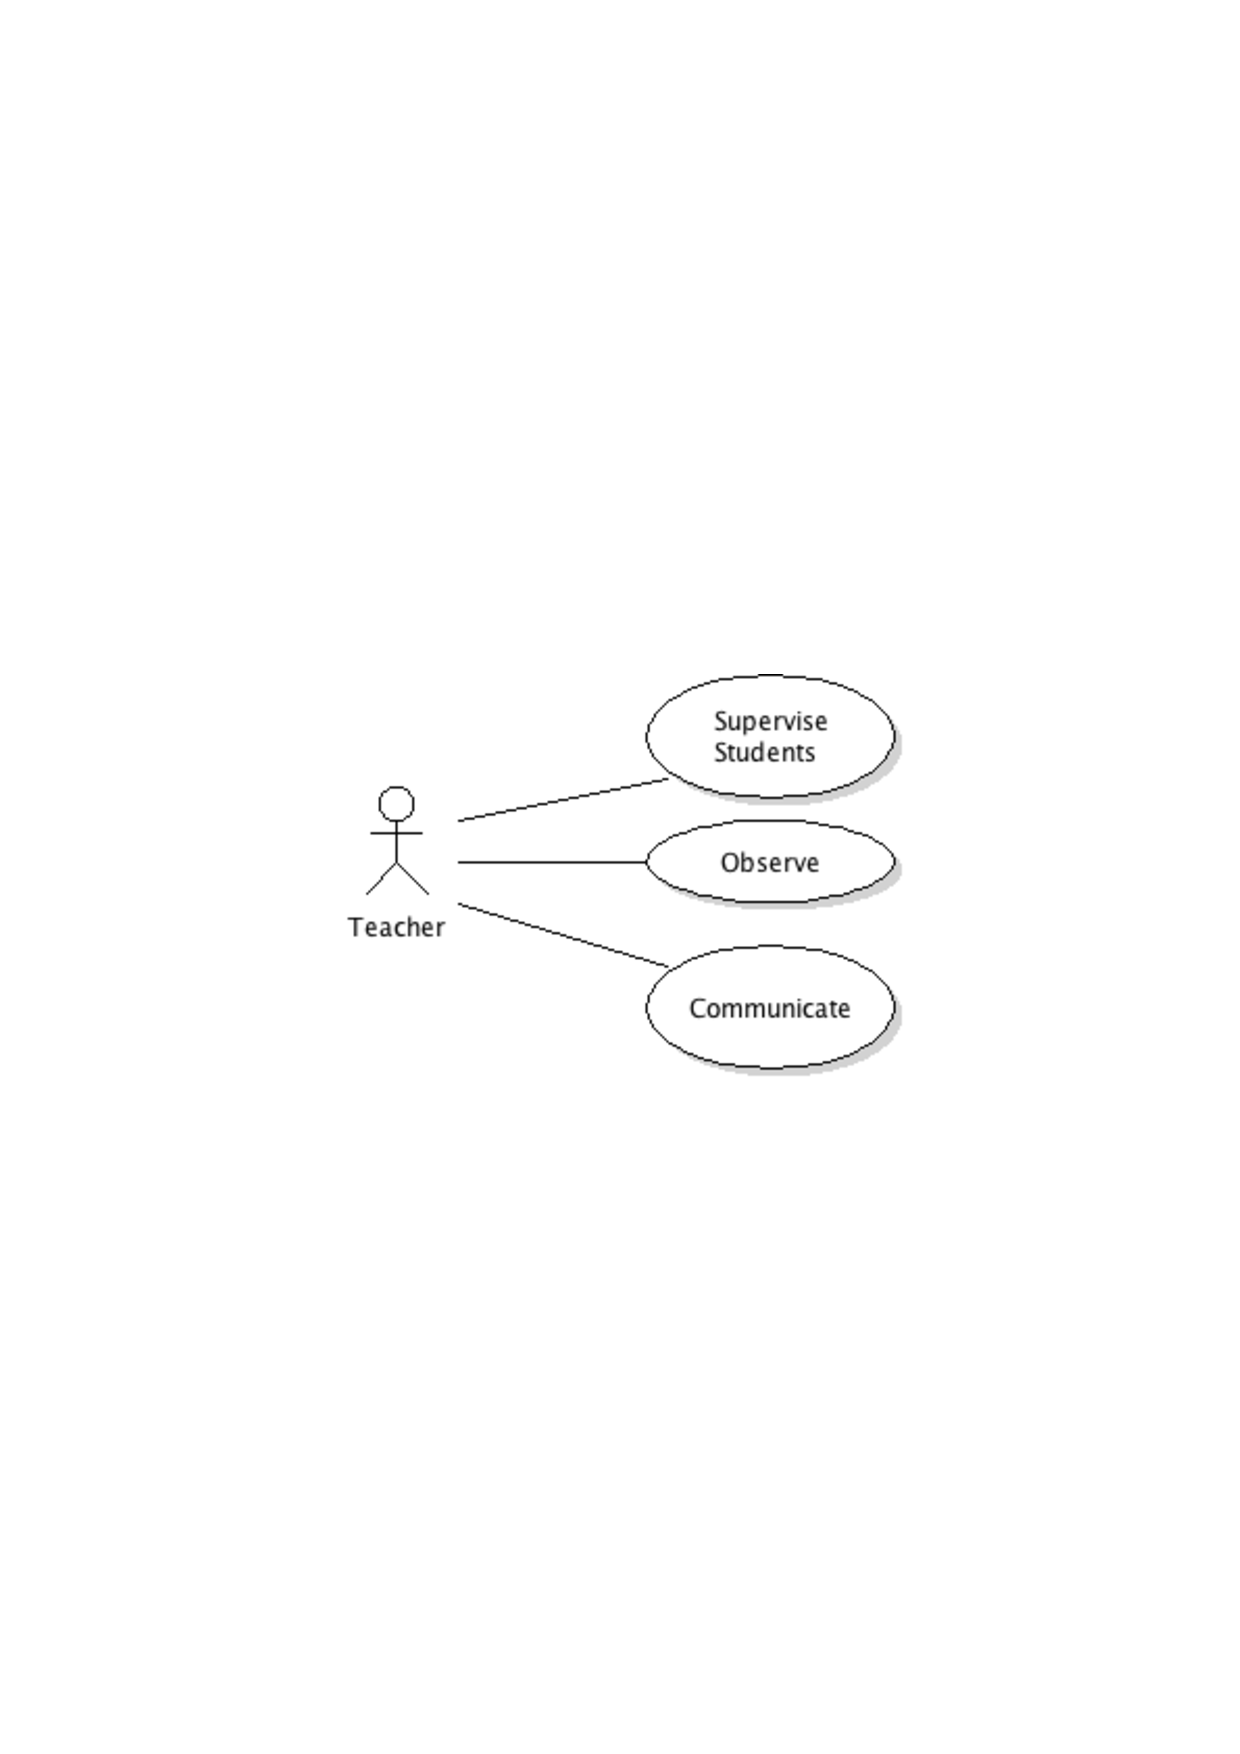
\includegraphics[width=\textwidth,  trim=2cm 11cm 2cm 12cm]{UML_figure/UC/teacher/UC_Teacher_General.pdf}
				\caption{Teacher use cases : Overview}
			\end{center}
		\end{figure}
		\subsubsection{Supervise students}
			The teacher supervises students by providing exercises and grading them.
		\subsubsection{Observe}
			The teacher observes students's grade and remediate to help them.
		\subsubsection{Communicate}
			The students communicates with authenticate users in order to fix her issue and to help students.
\newpage
	\subsection{Supervise students}
		\begin{figure}[ht]
			\begin{center}
				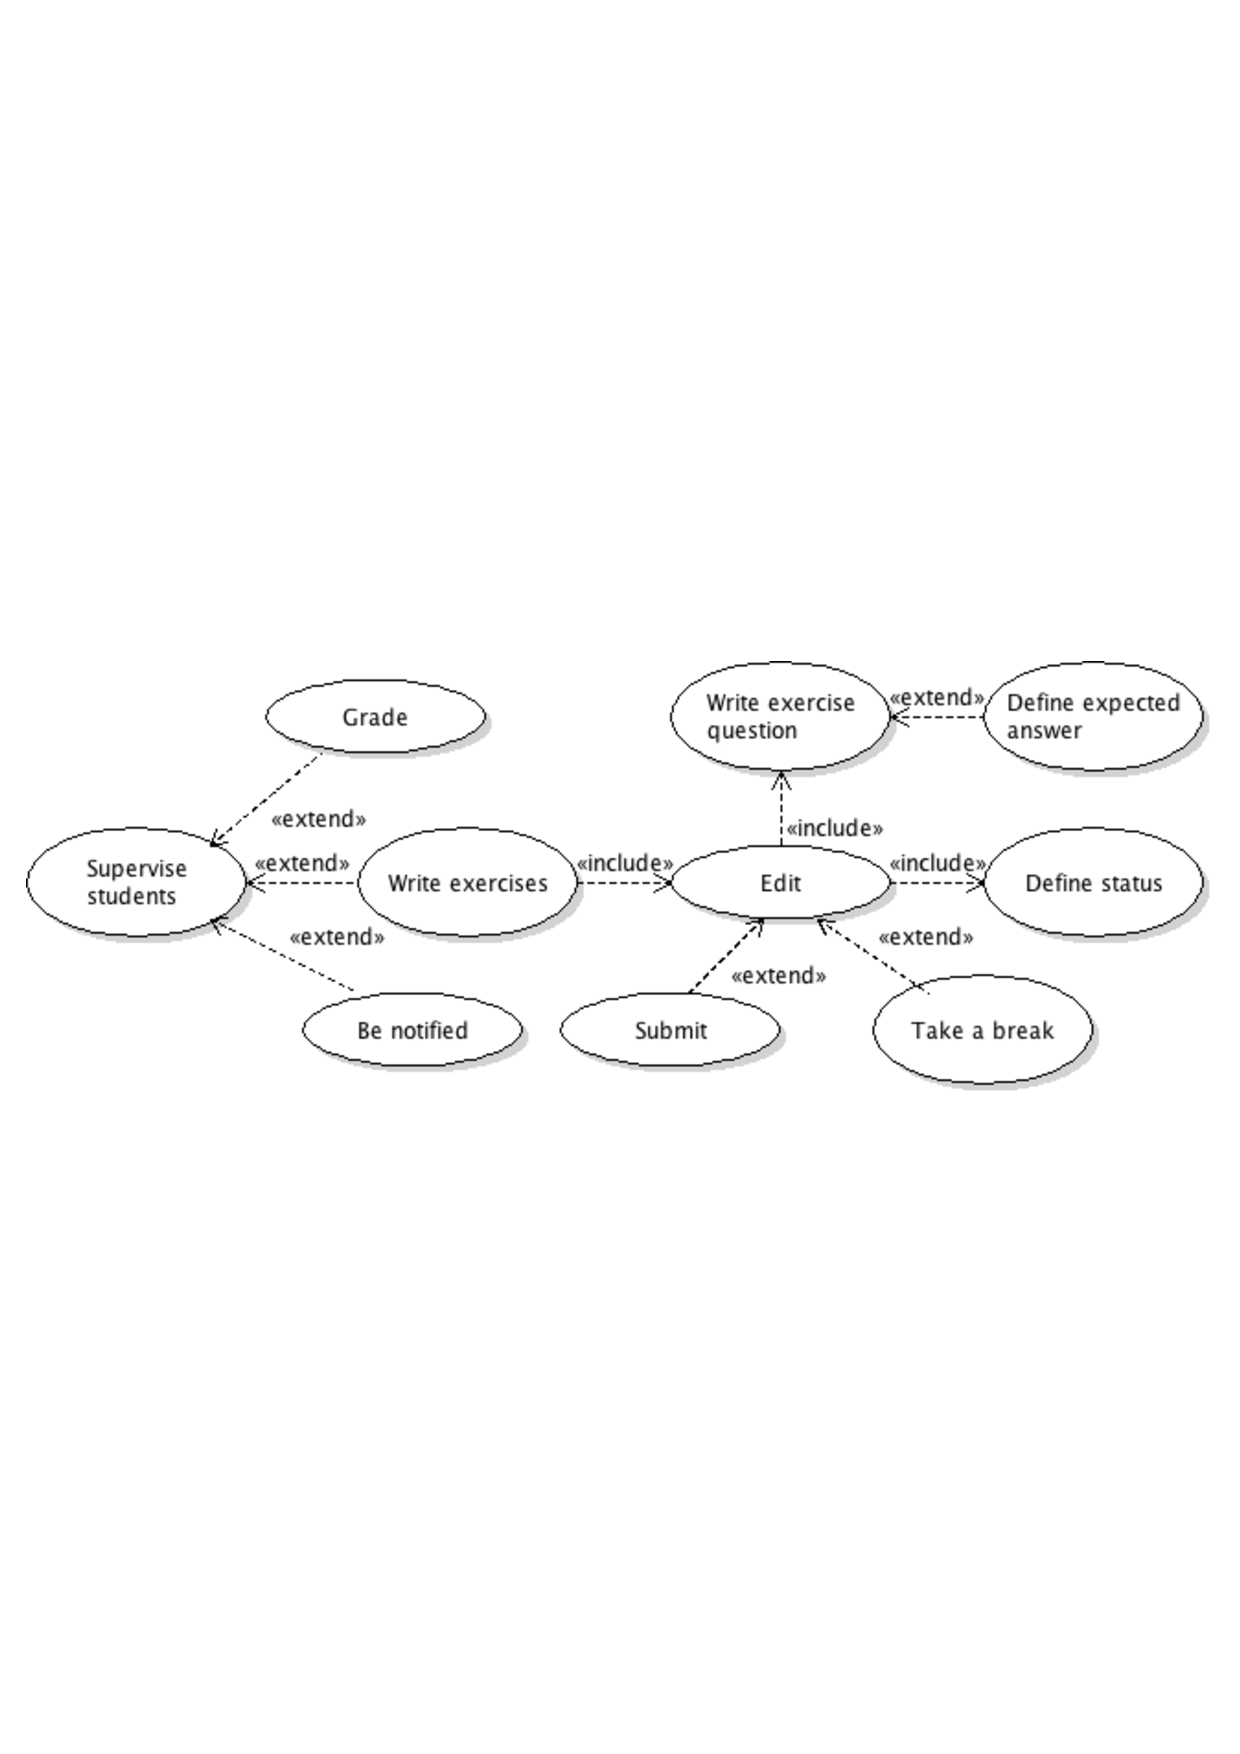
\includegraphics[width=\textwidth,  trim=2cm 10cm 2cm 10cm]{UML_figure/UC/teacher/UC_Teacher_Supervise.pdf}
				\caption{Teacher use cases : Supervise students}
			\end{center}
		\end{figure}
		\subsubsection{Grade}
			The teacher grades students answers for questions which have no fully-automatic grading system.
		\subsubsection{Be Notified}
			The teacher will be notified of events.
			For instance the teacher will be notified when one of her exercises is online.
		\subsubsection{Write exercises}
			The teacher writes exercise descriptions (statements, resources, ...).
		\subsubsection{Define expected answer}
			When the teacher writes exercises, he can optionally define an expected answer.
		\subsubsection{Edit}
			The teacher can edit any exercise at anytime.
		\subsubsection{Define Status}
			The teacher attaches a status to an exercise (date of release, condition of release, student concerned...) 
		\subsubsection{Take a break}
			The teacher can resume the edition of her exercise later.
		\subsubsection{Submit}
			The teacher submits her exercise which can be viewed by student according to the exercise status defined by the teacher.
	%\newpage
	\subsection{Observe}
		\begin{figure}[ht]
			\begin{center}
				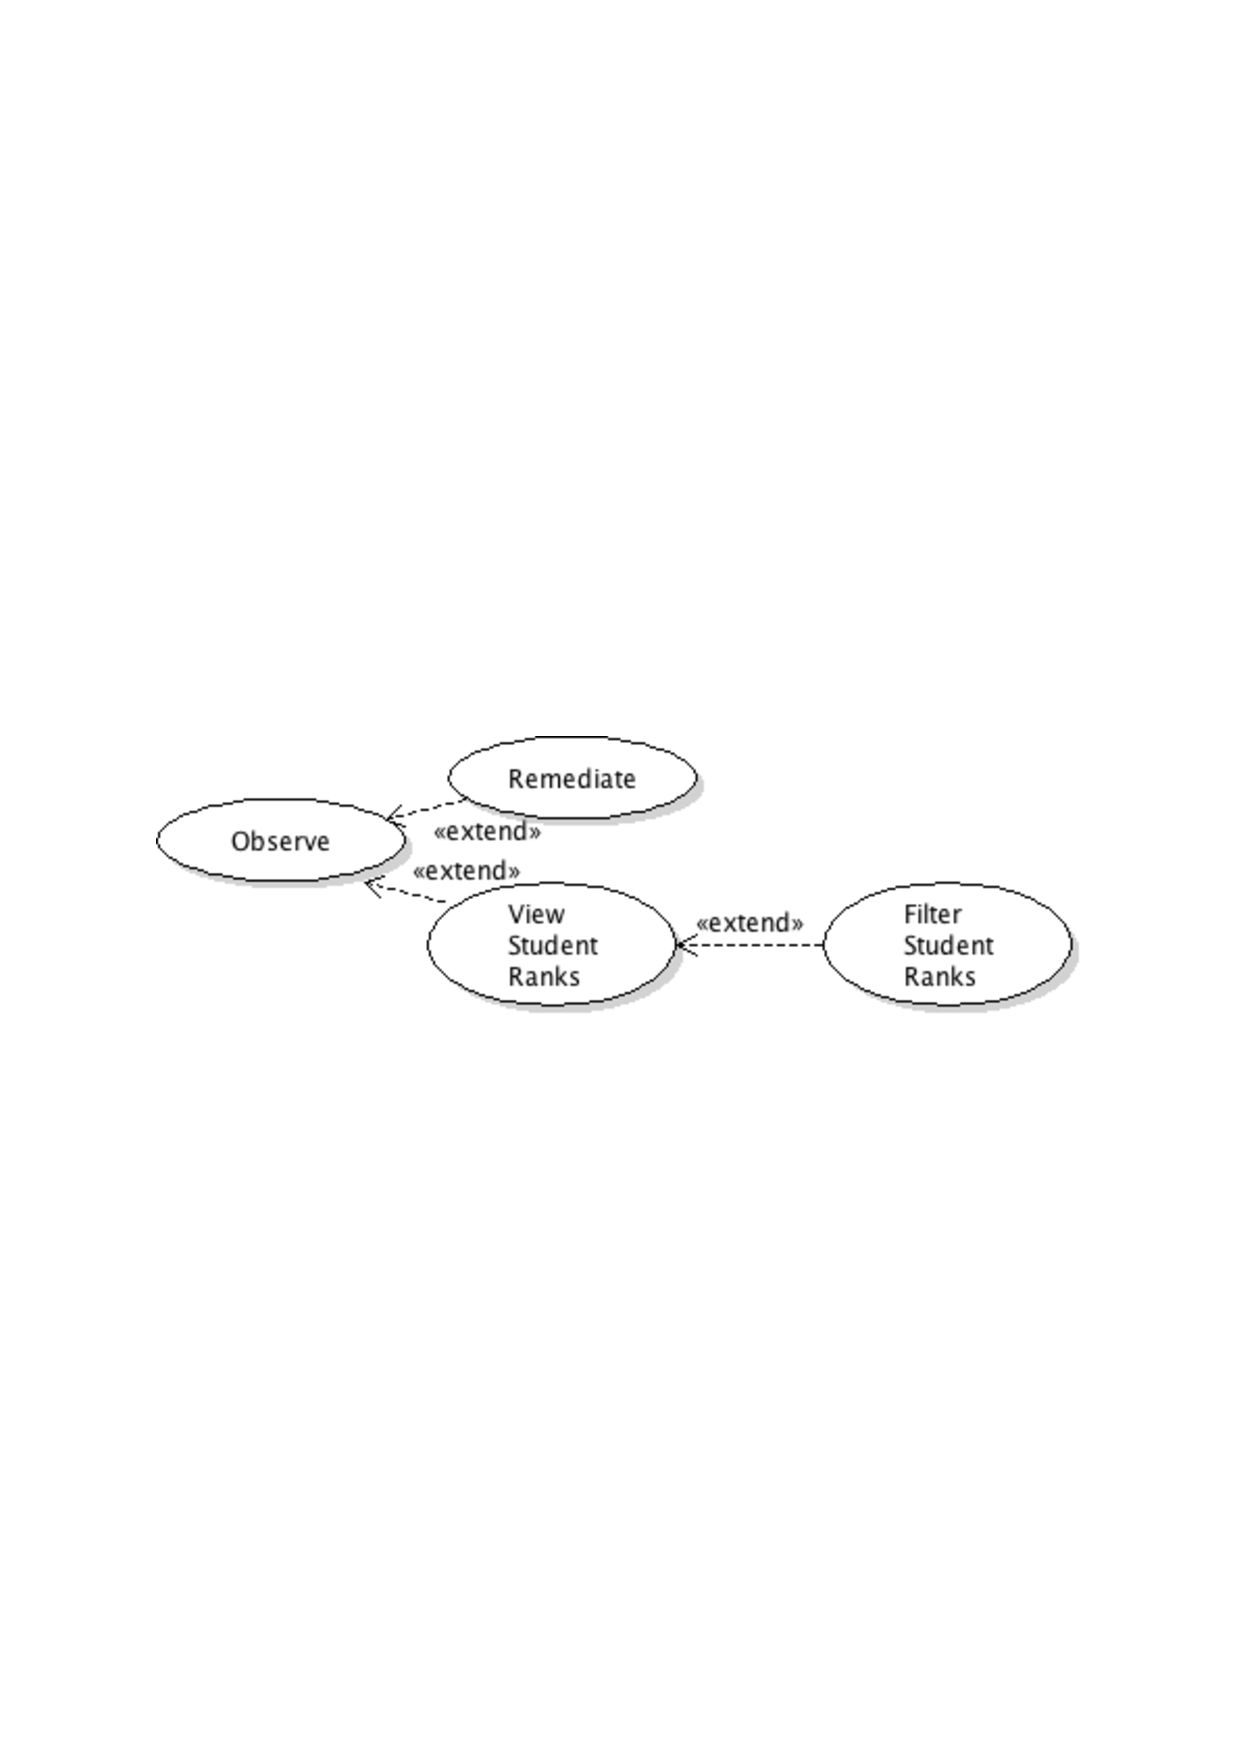
\includegraphics[width=\textwidth,  trim=2cm 12cm 2cm 12cm]{UML_figure/UC/teacher/UC_Teacher_Observe.pdf}
				\caption{Teacher use cases : Observe}
			\end{center}
		\end{figure}
		\subsubsection{View students ranks}
			The teacher observes all the grades of students who took his exercises.
		\subsubsection{Filter students ranks}
			The teacher filters the grades according to some critera.
			The criteria can be the identifier of a group or the year for instance.
		\subsubsection{Remediate}
			The teacher can provide exercises for a group of students in trouble with some specific subject of the course according to their grades.
%end teacher section
\newpage
%begin administrator section
\section{Administrator}
	\subsection{Overview}
		\begin{figure}[ht]
			\begin{center}
				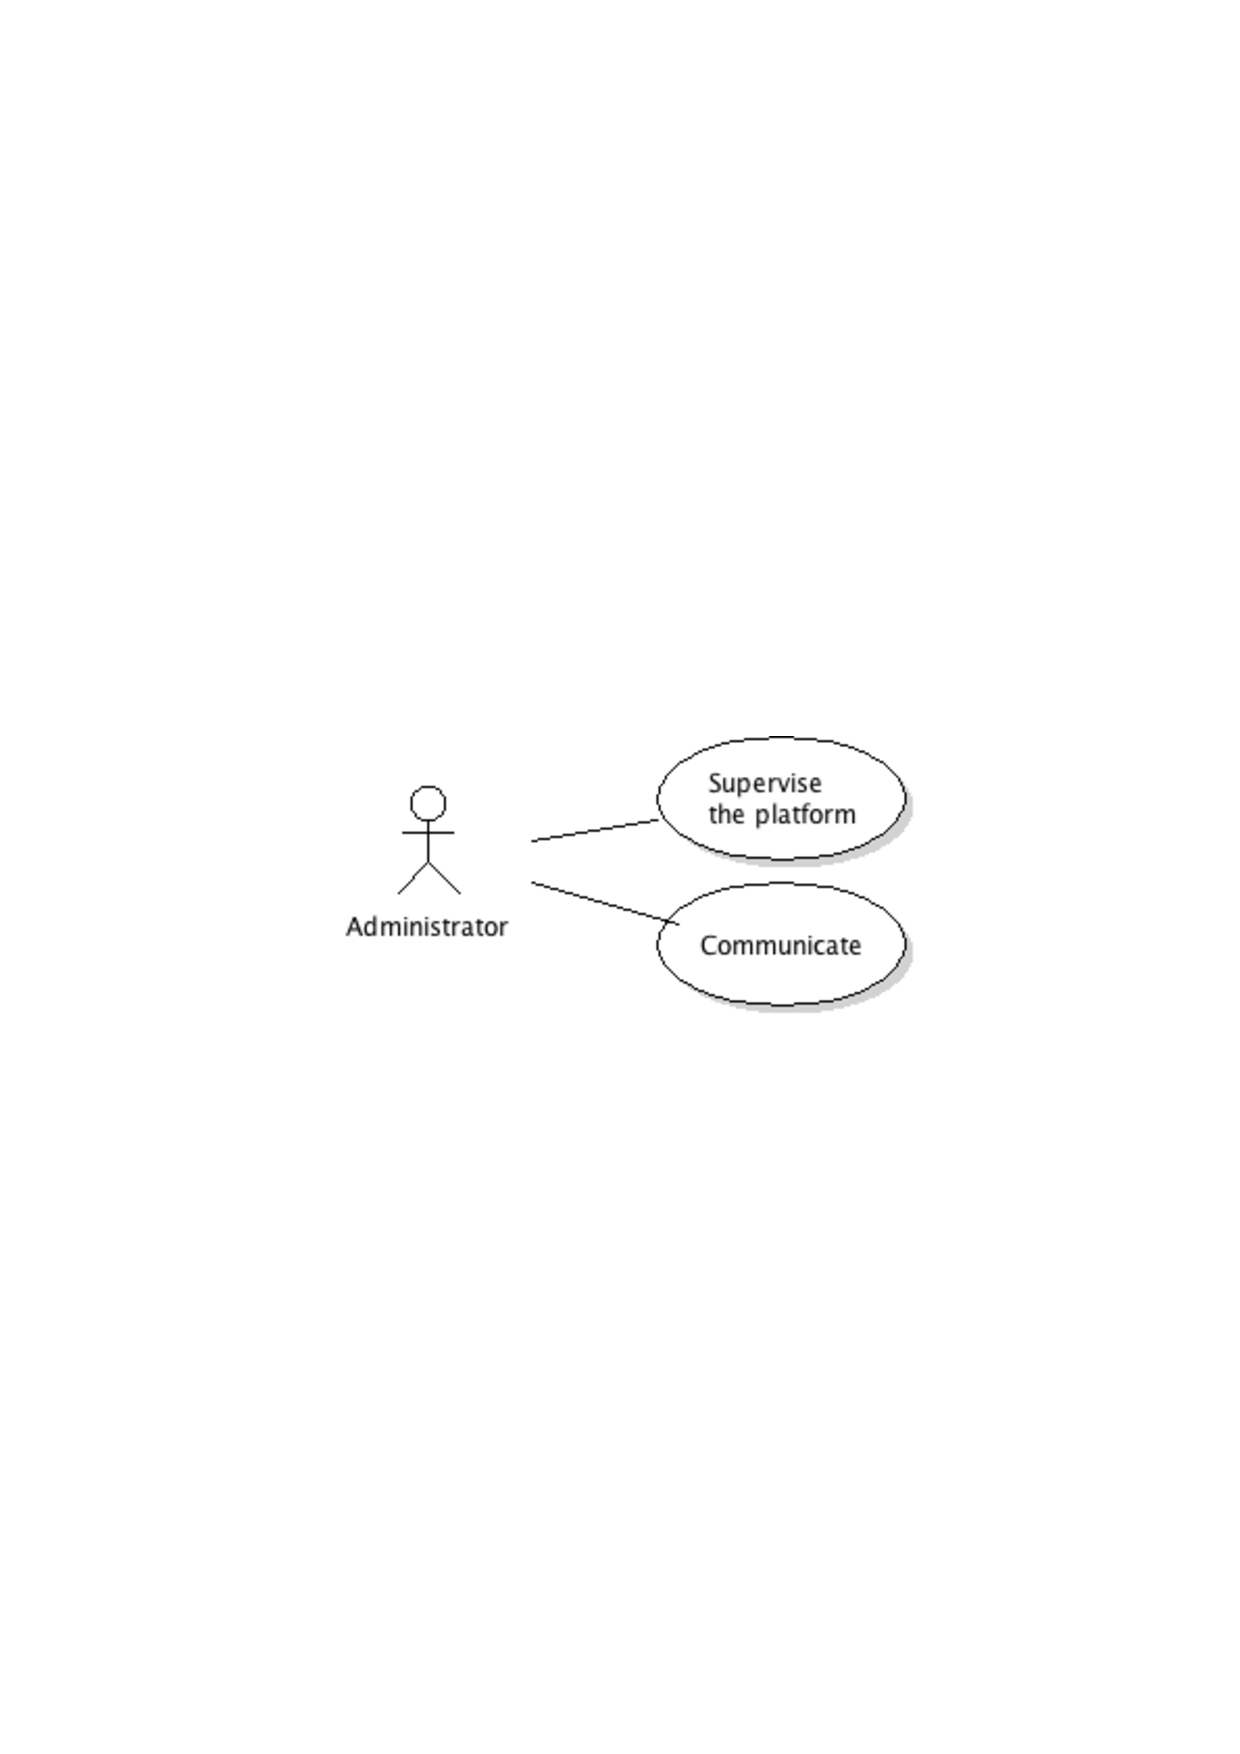
\includegraphics[width=\textwidth, trim=2cm 12cm 2cm 12cm]{UML_figure/UC/administrator/UC_Administrator_General.pdf}
				\caption{Administrator use cases : Overview}
			\end{center}
		\end{figure}
		\subsubsection{Supervise the platform}
			The administrator supervises the platform in order to ensure the platform operates smoothly.
		\subsubsection{Communicate}
			The administrator communicates with authenticate users in order to fix their issue.
	\subsection{Supervise the platform}
		\begin{figure}[ht]
			\begin{center}
				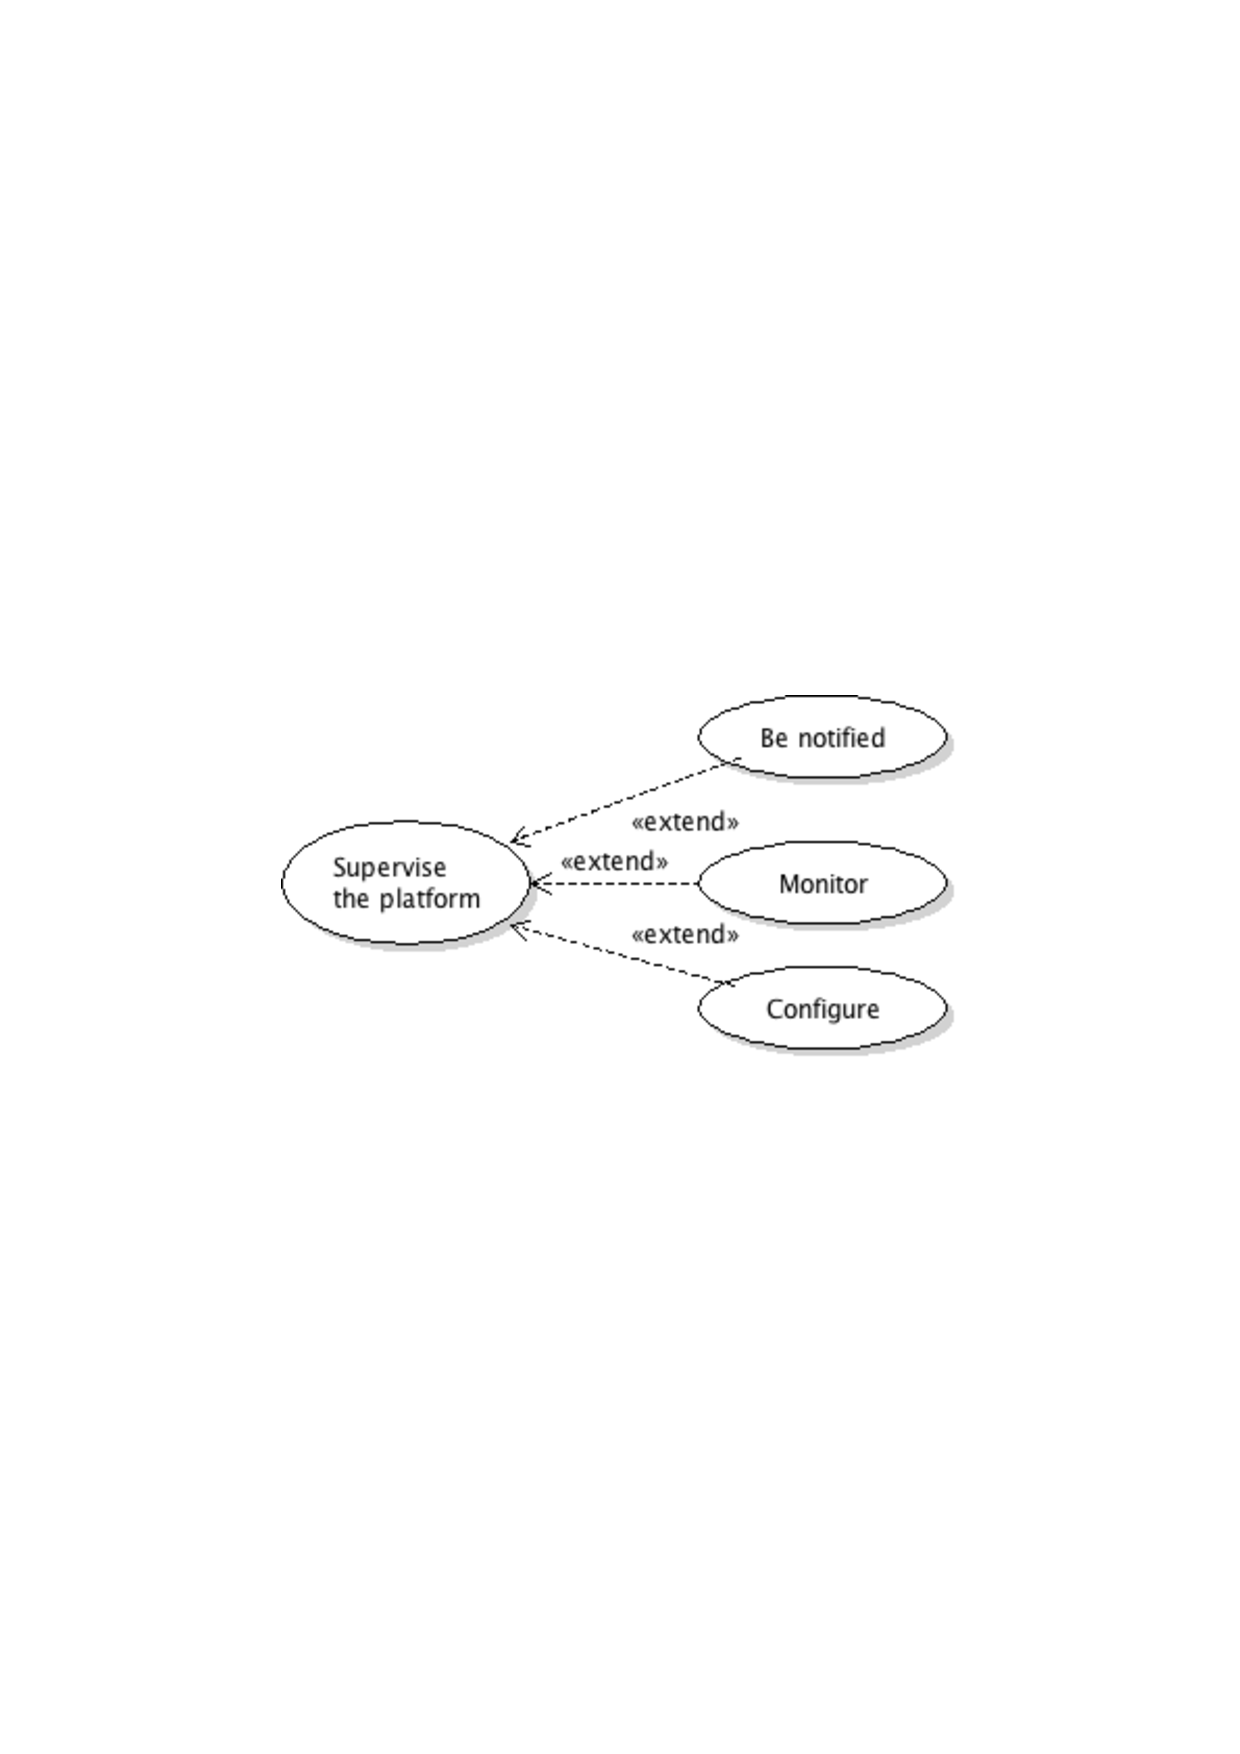
\includegraphics[width=\textwidth, trim=2cm 12cm 2cm 12cm]{UML_figure/UC/administrator/UC_Administrator_Supervise.pdf}
				\caption{Administrator use cases : Supervise the platform}
			\end{center}
		\end{figure}
		\subsubsection{Be notified}
			The administrator will be notified by events such as a critical issue.
		\subsubsection{Monitor}
			The administrator inspects the log in real time.
		\subsubsection{Configure}
			The administrator configures the platform.
%end administrator section
%begin common user section
\section{Common registered user}
	\begin{figure}[ht]
		\begin{center}
			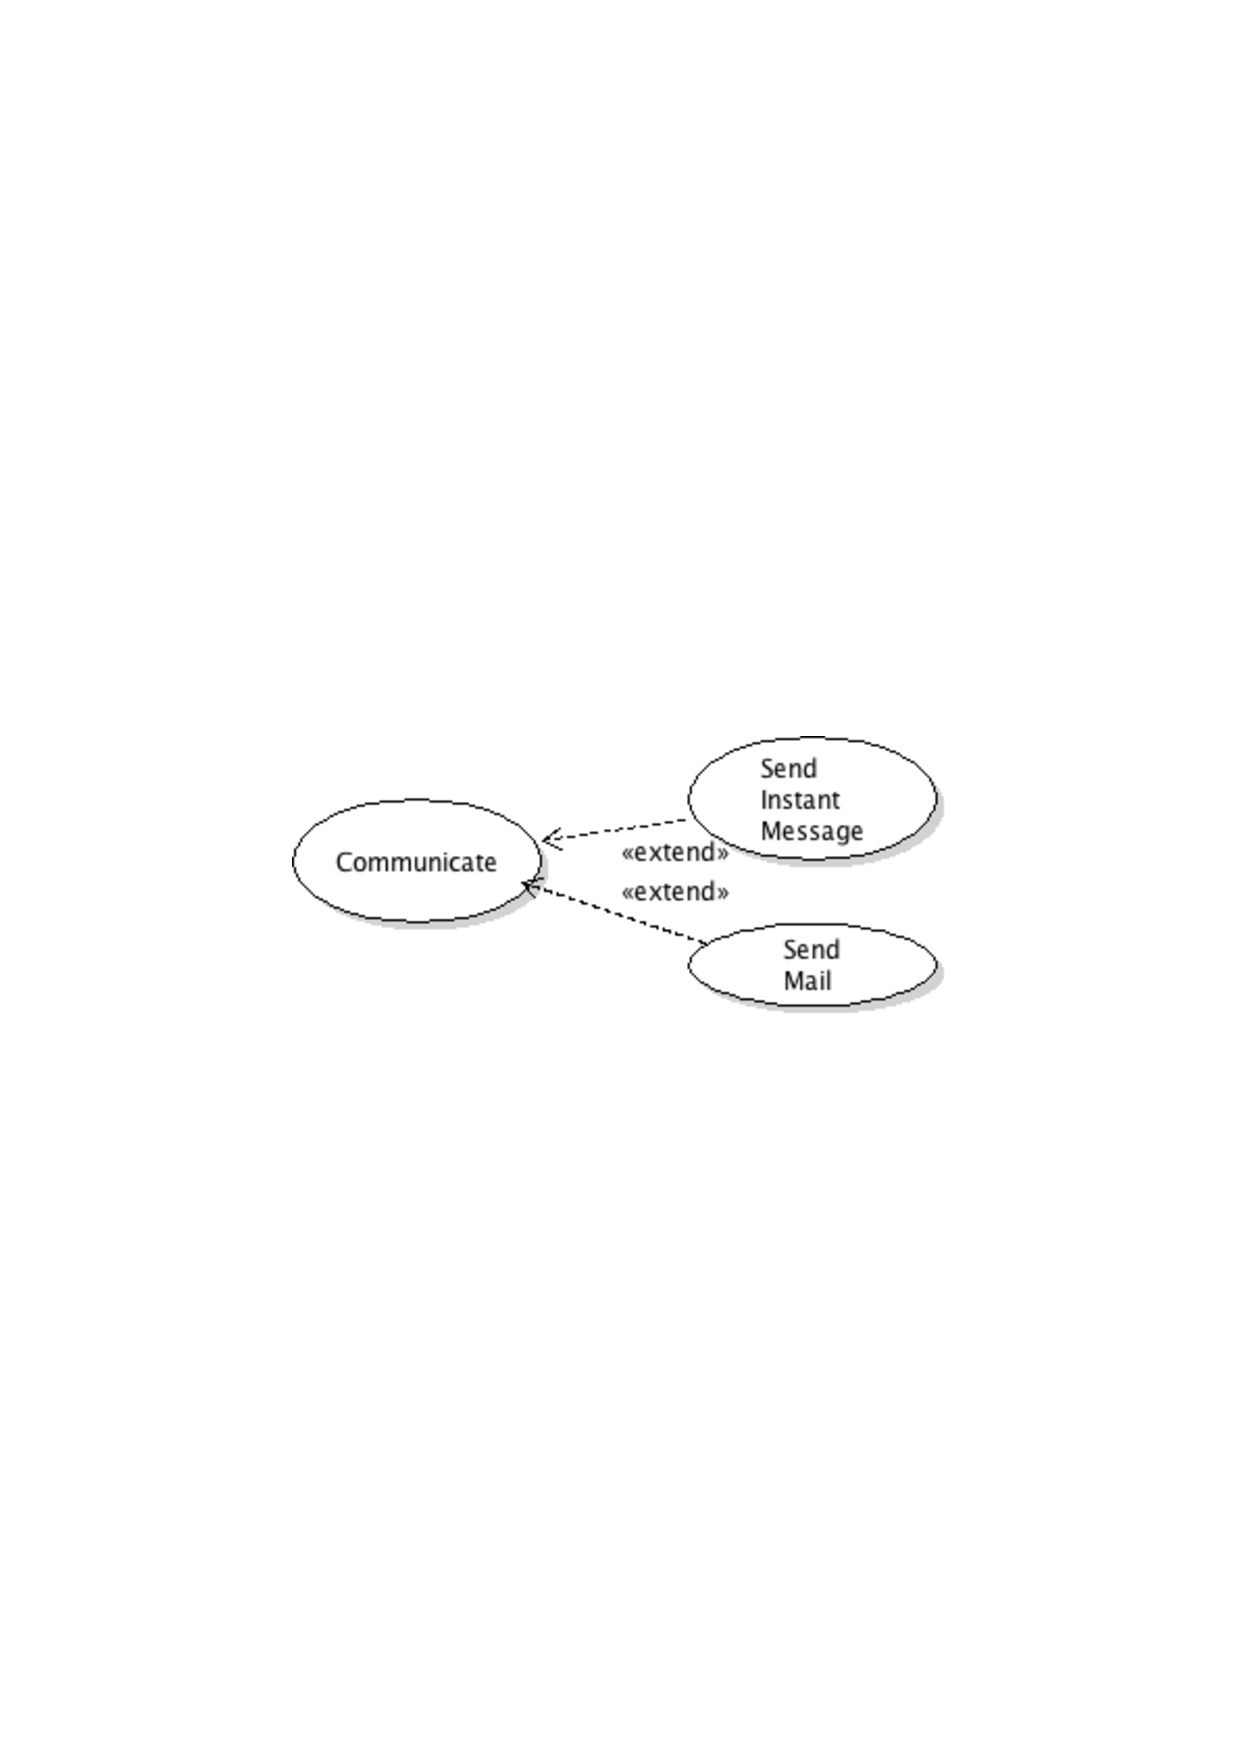
\includegraphics[width=\textwidth,  trim=2cm 12cm 2cm 12cm]{UML_figure/UC/common/UC_Common_Communicate.pdf}
			\caption{Registered user use cases : Communicate}
		\end{center}
	\end{figure}
	\subsubsection{Communicate}
		Identified user communicate between them through various message system provide by the platform.
	\subsubsection{Send Mail}
		Identifed user communicate by mail exchange.
	\subsubsection{Send Instant Message}
		Identifed user communicate by instant message exchange.
%end common user section
%end chapter useCase
